\documentclass[convert={outfile=\jobname.svg}]{standalone}
\usepackage[dvipsnames]{xcolor}
\usepackage{tikz}
\tikzset{dot/.style={draw,shape=circle,fill=black,scale=0.4}}

\begin{document}
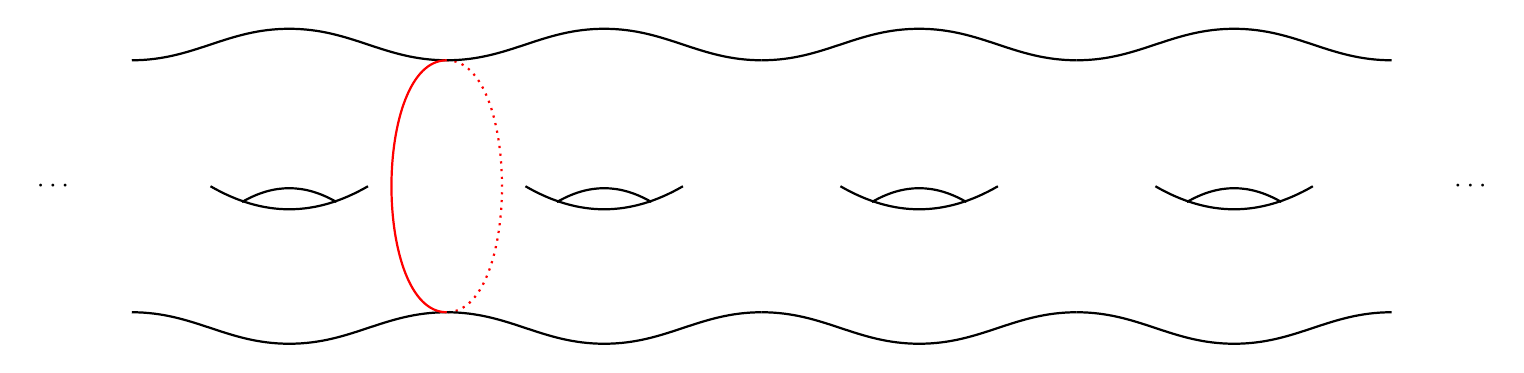
\begin{tikzpicture}[scale=2, thick]
    \draw [red, dotted] (-6, 0.8) to [out=0,in=0, looseness=0.75] (-6, -0.8);
    
    % Left.
    \foreach \i in {-6, -4, -2, 0} {
    \begin{scope}[shift={(\i, 0)}]
    \draw (0, 0.8)
        to [out=180,in=0] (-1, 1)
        to [out=180,in=0] (-2, 0.8);
    
    \draw (-2, -0.8)
        to [out=0,in=180] (-1, -1)
        to [out=0,in=180] (0, -0.8);
    
    \draw (-1.5,0) to [out=-30,in=180+30] (-0.5,0);
    \draw (-1.3,-0.1) to [out=30,in=180-30] (-0.7,-0.1);
    \end{scope}
    }
    \draw [red] (-6, 0.8) to [out=180,in=180, looseness=0.75] (-6, -0.8);
    
    \node at (0.5, 0) {$\cdots$};
    \node at (-8.5, 0) {$\cdots$};
\end{tikzpicture}
\end{document}
